% Options for packages loaded elsewhere
\PassOptionsToPackage{unicode}{hyperref}
\PassOptionsToPackage{hyphens}{url}
\documentclass[
  11pt,
]{article}
\usepackage{xcolor}
\usepackage{amsmath,amssymb}
\setcounter{secnumdepth}{-\maxdimen} % remove section numbering
\usepackage{iftex}
\ifPDFTeX
  \usepackage[T1]{fontenc}
  \usepackage[utf8]{inputenc}
  \usepackage{textcomp} % provide euro and other symbols
\else % if luatex or xetex
  \usepackage{unicode-math} % this also loads fontspec
  \defaultfontfeatures{Scale=MatchLowercase}
  \defaultfontfeatures[\rmfamily]{Ligatures=TeX,Scale=1}
\fi
\usepackage{lmodern}
\ifPDFTeX\else
  % xetex/luatex font selection
\fi
% Use upquote if available, for straight quotes in verbatim environments
\IfFileExists{upquote.sty}{\usepackage{upquote}}{}
\IfFileExists{microtype.sty}{% use microtype if available
  \usepackage[]{microtype}
  \UseMicrotypeSet[protrusion]{basicmath} % disable protrusion for tt fonts
}{}
\makeatletter
\@ifundefined{KOMAClassName}{% if non-KOMA class
  \IfFileExists{parskip.sty}{%
    \usepackage{parskip}
  }{% else
    \setlength{\parindent}{0pt}
    \setlength{\parskip}{6pt plus 2pt minus 1pt}}
}{% if KOMA class
  \KOMAoptions{parskip=half}}
\makeatother
\usepackage{longtable,booktabs,array}
\usepackage{caption}
\captionsetup[table]{skip=6pt}
\newcounter{none} % for unnumbered tables
\usepackage{calc} % for calculating minipage widths
% Correct order of tables after \paragraph or \subparagraph
\usepackage{etoolbox}
\makeatletter
\patchcmd\longtable{\par}{\if@noskipsec\mbox{}\fi\par}{}{}
\makeatother
% Allow footnotes in longtable head/foot
\IfFileExists{footnotehyper.sty}{\usepackage{footnotehyper}}{\usepackage{footnote}}
\makesavenoteenv{longtable}
\setlength{\emergencystretch}{3em} % prevent overfull lines
\providecommand{\tightlist}{%
  \setlength{\itemsep}{0pt}\setlength{\parskip}{0pt}}
% ===== 中文与字体 =====
\usepackage[UTF8]{ctex}
\setCJKmonofont{SimHei}
% 等宽字体需支持制表符（流程图用），Latin Modern Mono 不含 U+2500 区段
\setmonofont{Consolas}[Scale=0.88]

% ===== 页面 =====
\usepackage{geometry}
\geometry{a4paper, top=2.6cm, bottom=2.6cm, left=2.6cm, right=2.6cm}

% ===== 行距与段落 =====
\linespread{1.32}
\setlength{\parskip}{0.35em}
\setlength{\parindent}{2em}

% ===== 表格 =====
\usepackage{longtable,booktabs,array}
\usepackage{needspace}
\renewcommand{\arraystretch}{1.32}
\setlength{\LTpre}{8pt}
\setlength{\LTpost}{8pt}

% ===== 代码块 =====
\usepackage{fancyvrb}
\fvset{fontsize=\small}

% ===== 页眉页脚 =====
\usepackage{fancyhdr}
\pagestyle{fancy}
\fancyhf{}
\fancyhead[L]{\small\songti AI 生成 PPT 的最后一公里}
\fancyhead[R]{\small\songti 项目报告}
\fancyfoot[C]{\small\thepage}
\renewcommand{\headrulewidth}{0.4pt}
\fancypagestyle{plain}{\fancyhf{}\fancyfoot[C]{\small\thepage}\renewcommand{\headrulewidth}{0pt}}

% ===== 链接颜色 =====
\usepackage{xcolor}
\usepackage{xurl}
\usepackage{hyperref}
\definecolor{linkblue}{HTML}{185FA5}
\definecolor{rulegray}{HTML}{888780}
\hypersetup{colorlinks=true, linkcolor=linkblue, urlcolor=linkblue, citecolor=linkblue}

% ===== 节标题样式 =====
\usepackage{titlesec}
\titleformat{\section}{\Large\heiti}{\thesection}{0.8em}{}
\titleformat{\subsection}{\large\heiti}{\thesubsection}{0.7em}{}
\titlespacing*{\section}{0pt}{1.6em}{0.7em}
\titlespacing*{\subsection}{0pt}{1.1em}{0.5em}

% ===== 图表标题 =====
\usepackage{caption}
\captionsetup{font=small,labelsep=quad}

% ===== 图 =====
\usepackage{tikz}
\usetikzlibrary{arrows.meta,positioning,calc}

% ===== 公式间距 =====
\AtBeginDocument{%
  \setlength{\abovedisplayskip}{9pt plus 2pt minus 1pt}%
  \setlength{\belowdisplayskip}{11pt plus 2pt minus 1pt}%
  \setlength{\abovedisplayshortskip}{5pt}%
  \setlength{\belowdisplayshortskip}{7pt}%
}

% ===== 避免表格跨页孤行 =====
\widowpenalty=10000
\clubpenalty=10000

% ===== 标题页与目录独立成页 =====
\let\pandocmk\maketitle
\renewcommand{\maketitle}{\pandocmk\thispagestyle{empty}\newpage}
\let\pandoctoc\tableofcontents
\renewcommand{\tableofcontents}{\pandoctoc\newpage}
\usepackage{bookmark}
\IfFileExists{xurl.sty}{\usepackage{xurl}}{} % add URL line breaks if available
\urlstyle{same}
% fallback for those not using the hyperref driver hyperxmp:
\makeatletter
\@ifundefined{xmpquote}{\newcommand{\xmpquote}[1]{#1}}{}
\makeatother
\hypersetup{
  pdftitle={AI 生成 PPT 的最后一公里},
  hidelinks,
  pdfcreator={LaTeX via pandoc}}

\title{AI 生成 PPT 的最后一公里}
\usepackage{etoolbox}
\makeatletter
\providecommand{\subtitle}[1]{% add subtitle to \maketitle
  \apptocmd{\@title}{\par {\large #1 \par}}{}{}
}
\makeatother
\subtitle{面向 AI 生成演示文稿的多层质量审查与按需复核智能体}
\author{}
\date{2026 年 10 月}

\begin{document}
\maketitle

{
\setcounter{tocdepth}{1}
\tableofcontents
}
\section{项目概览}\label{ux9879ux76eeux6982ux89c8}

{\def\LTcaptype{none} % do not increment counter
\begin{longtable}[]{@{}
  >{\raggedright\arraybackslash}p{(\linewidth - 2\tabcolsep) * \real{0.1964}}
  >{\raggedright\arraybackslash}p{(\linewidth - 2\tabcolsep) * \real{0.8036}}@{}}
\toprule\noalign{}
\begin{minipage}[b]{\linewidth}\raggedright
项
\end{minipage} & \begin{minipage}[b]{\linewidth}\raggedright
内容
\end{minipage} \\
\midrule\noalign{}
\endhead
\bottomrule\noalign{}
\endlastfoot
项目名称 & AI 生成 PPT 的最后一公里 \\
项目正式名 & 基于多层协同检测与按需复核的 PPT
质量审查智能体设计与实现 \\
课程 & 《智能体设计》期末项目（八周） \\
项目类型 & 融合确定性规则、传统机器学习与多模态大模型的智能交互系统 \\
主要用户 & 使用生成式 AI 制作 PPT 的高校学生、教师、科研与办公人员 \\
核心对象 & AI 生成的演示文稿，优先支持可编辑 PPTX \\
报告日期 & 2026 年 10 月 \\
\end{longtable}
}

\section{摘要}\label{ux6458ux8981}

生成式 AI
已能把演示文稿的制作成本从数小时压缩到数分钟，却没有压缩交付前的验收成本。用户拿到一份
AI
生成稿后，仍需逐页核对排版、字体、数据一致性、内容覆盖度，这部分工作被称为''最后一公里''。

本项目构建一套面向该场景的质量审查系统。系统以可编辑 PPTX
为输入，通过结构解析与页面渲染获得两类证据；以确定性规则处理几何与属性问题，以轻量视觉分类器处理模糊的排版判定，以多模态大模型处理语义级问题；在融合层对多源结论去重、分档、冲突降级，并按置信度决定是否追加一次模型复核；最终输出一份每条结论可回溯到具体元素、每条建议可落到具体操作的风险与优化报告。

系统的技术要点有三：其一，检测路由由缺陷类别表显式给定，而非由编码前缀推断，使''视觉现象但结构可判''的缺陷能走低成本路径；其二，将''AI
风格痕迹''分解为页内的 PTPS 与页间的 HCI
两个可计算指标，明确不输出生成概率；其三，把大模型调用次数作为一等实验指标，与分类别准确率一同报告，用于回答''哪些缺陷值得调用模型''这一成本问题。

本报告说明问题边界、系统架构、关键方法、数据与模型方案、课程知识映射、分阶段开发路线，以及已知风险与局限。

\section{1
项目背景与问题定义}\label{ux9879ux76eeux80ccux666fux4e0eux95eeux9898ux5b9aux4e49}

\subsection{1.1
成本被转移，而不是被消除}\label{ux6210ux672cux88abux8f6cux79fbux800cux4e0dux662fux88abux6d88ux9664}

生成式 AI
对演示文稿的改变，发生在''从无到有''这一段：一句话生成一份结构完整的初稿，过去需要数小时，现在需要数分钟。

但交付前的验收并没有随之消失，只是从''制作''转移到了''检查''。一份十五页的
AI 生成稿，用户通常需要完成以下核对：

\begin{itemize}
\tightlist
\item
  页面排版是否正常，有无文字溢出、元素越界、遮挡压字；
\item
  视觉风格是否统一，字号层级是否清晰；
\item
  装饰性元素（图标、emoji、渐变块）是否过多且无信息功能；
\item
  不同页面之间的关键数据、术语、结论是否一致；
\item
  生成结果是否满足最初的制作要求，是否覆盖了参考资料的关键内容；
\item
  在时间有限的前提下，哪几页真正值得改。
\end{itemize}

这项工作单条不难，但条目多、易遗漏、且难以委托给任何单一工具：规则看不出语义矛盾，大模型说不清元素坐标。

\subsection{1.2 核心问题}\label{ux6838ux5fc3ux95eeux9898}

\begin{quote}
如何通过规则、传统机器学习与多模态大模型的协同，把''逐页人工验收''压缩为''读一份报告并处理若干条建议''，同时保证每条结论有据可查、每条建议可以直接执行？
\end{quote}

该问题可拆为三个可独立回答的子问题：

{\def\LTcaptype{none} % do not increment counter
\begin{longtable}[]{@{}lll@{}}
\toprule\noalign{}
子问题 & 关注点 & 对应设计 \\
\midrule\noalign{}
\endhead
\bottomrule\noalign{}
\endlastfoot
哪些缺陷不需要模型就能判定 & 成本 & 分层检测与检测路由 \\
判定一类缺陷需要什么证据 & 可靠性 & 证据族与统一记录结构 \\
报告写到什么程度用户才敢照着改 & 可用性 & 三级可执行建议 \\
\end{longtable}
}

\subsection{1.3 项目边界}\label{ux9879ux76eeux8fb9ux754c}

边界不是免责声明，而是设计约束。以下五条在全项目中不可放松：

\begin{enumerate}
\def\labelenumi{\arabic{enumi}.}
\tightlist
\item
  \textbf{不判定 PPT 是否由 AI 生成}，不输出任何形式的生成概率或''AI
  率''。
\item
  \textbf{不核验内容的事实真伪}，只核验与用户提供的参考资料之间的一致性。
\item
  \textbf{不自动修改用户文件}。系统给出定位、数值与操作路径，修改由用户执行。
\item
  \textbf{不在缺少证据时给出确定结论}。证据不足即标记为待人工核实。
\item
  \textbf{不宣称具备完全自主的规划能力}。自主性仅体现在''按需复核''这一处，且有成本上限。
\end{enumerate}

第一条需要展开一点：判断''是否由 AI 生成''在技术上要求一个以''AI
生成样本 vs
人工样本''为基线的判别模型，需要两类各数百份的标注数据。本项目不具备该条件，也不认为这是用户真正关心的问题------用户关心的是''这页做得像不像模板套出来的''，而不是''它的作者是谁''。

\section{2
相关工作与差异化定位}\label{ux76f8ux5173ux5de5ux4f5cux4e0eux5deeux5f02ux5316ux5b9aux4f4d}

\subsection{2.1 已有工作}\label{ux5df2ux6709ux5de5ux4f5c}

{\def\LTcaptype{none} % do not increment counter
\begin{longtable}[]{@{}
  >{\raggedright\arraybackslash}p{(\linewidth - 4\tabcolsep) * \real{0.2727}}
  >{\raggedright\arraybackslash}p{(\linewidth - 4\tabcolsep) * \real{0.3636}}
  >{\raggedright\arraybackslash}p{(\linewidth - 4\tabcolsep) * \real{0.3636}}@{}}
\toprule\noalign{}
\begin{minipage}[b]{\linewidth}\raggedright
工作
\end{minipage} & \begin{minipage}[b]{\linewidth}\raggedright
做了什么
\end{minipage} & \begin{minipage}[b]{\linewidth}\raggedright
与本项目的关系
\end{minipage} \\
\midrule\noalign{}
\endhead
\bottomrule\noalign{}
\endlastfoot
SlideAudit {[}1{]} & 2,400 张带设计缺陷标注的幻灯片图像（约 600 原始 +
1,800 变体）；评测多个多模态模型识别缺陷的能力 &
实验一的唯一监督数据来源；其报告的低 F1
是''单一大模型不足''的直接论据 \\
PPTEval {[}2{]} & 随 PPTAgent
一并提出，用大模型从内容、设计、连贯性三个维度为生成结果打 1--5 分 &
只给分数，不定位到元素，建议不可执行 \\
PresentBench {[}3{]} & 238 个 PPT 生成任务，每个任务配平均 54 条二元
checklist &
借鉴其''将自然语言要求拆成可核验条目''的做法，不作为训练数据 \\
AI Is Not Enough {[}4{]} & 用启发式从视图层级提取属性，结合设计规范 RAG
与大模型判定界面合规性 & 最接近的先例，证明''规则 +
大模型''的混合路线可行 \\
\end{longtable}
}

引用编号对应文末参考文献。需要说明的是，SlideAudit 的缺陷标签分为
\texttt{design\_deficiency\_category} 与 \texttt{design\_deficiency}
两级，本项目不预设其取值与本项目编码的对应关系，映射须在数据核查阶段逐条比对方可确定（见
5.3）。

\subsection{2.2 差异化定位}\label{ux5deeux5f02ux5316ux5b9aux4f4d}

SlideAudit
的结论值得单独强调：作者用多个大模型、多种提示策略识别幻灯片设计缺陷，报告的
F1 仅为 0.331 至
0.655，并在摘要中指出模型难以准确定位设计缺陷。这一结果同时构成两件事------它是本项目''必须分层''的论据，也意味着''让多模态模型审
PPT''这件事已有人做过。

因此本项目的差异不能建立在''我做了分层框架''上。可辩护的差异只有三处，且都能用指标证明：

\textbf{第一，把成本作为一等指标。}
现有工作报告的是准确率，很少回答''哪些缺陷值得调用大模型''。本项目将调用次数与
token 消耗与分类别准确率并列报告，绘制成本---效果曲线。

\textbf{第二，证据强制绑定。}
每条结论必须携带至少一条可回溯的证据引用（结构坐标、渲染区域或要求条目编号），空证据的记录在数据结构层面不允许存在。由此可以统计''无依据断言比例''这一指标。

\textbf{第三，落在可编辑 PPTX 的结构证据上。} SlideAudit
提供的坐标是从图像反推的，不是原生结构；因此在其上无法验证''规则层''的价值。本项目以可编辑
PPTX 为主对象，才能讨论''结构证据让哪些判断变便宜''。

\section{3 系统架构}\label{ux7cfbux7edfux67b6ux6784}

\subsection{3.1 总体分层}\label{ux603bux4f53ux5206ux5c42}

系统分为六层，前四层在本地执行，第五层按需调用，第六层呈现结果。

\needspace{9\baselineskip}

{\def\LTcaptype{none} % do not increment counter
\begin{longtable}[]{@{}
  >{\raggedright\arraybackslash}p{(\linewidth - 6\tabcolsep) * \real{0.0536}}
  >{\raggedright\arraybackslash}p{(\linewidth - 6\tabcolsep) * \real{0.2143}}
  >{\raggedright\arraybackslash}p{(\linewidth - 6\tabcolsep) * \real{0.5357}}
  >{\raggedright\arraybackslash}p{(\linewidth - 6\tabcolsep) * \real{0.1964}}@{}}
\toprule\noalign{}
\begin{minipage}[b]{\linewidth}\raggedright
层
\end{minipage} & \begin{minipage}[b]{\linewidth}\raggedright
名称
\end{minipage} & \begin{minipage}[b]{\linewidth}\raggedright
主要职责
\end{minipage} & \begin{minipage}[b]{\linewidth}\raggedright
是否调用模型
\end{minipage} \\
\midrule\noalign{}
\endhead
\bottomrule\noalign{}
\endlastfoot
L0 & 输入与预处理 & PPTX 解析、页面渲染、文字与图像特征提取 & 否 \\
L1 & 规则检测 & 几何、字号、越界、页数、装饰计数 & 否 \\
L2 & 机器学习检测 & 针对模糊排版判定的视觉分类器 & 否（本地推理） \\
L3 & 风格分析 & 页内 PTPS、页间 HCI & 否 \\
L4 & 语义与要求核验 & 跨页一致性、图文关系、参考资料覆盖 & 是 \\
L5 & 调度、融合与报告 & 路由、复核、去重、分档、报告生成 & 视复核而定 \\
\end{longtable}
}

L0 与 L1 的处理单元是 PPTX 对象，L2 与 L3
的处理单元是渲染图与页级特征，L4 的处理单元是页面文本与图像，L5
的处理单元是结论记录。

这一划分有一条物理依据：\textbf{不同的缺陷能在不同证据上被判定}。文字是否越界只需读
XML
坐标，留白是否失衡需要看渲染图，两个数字是否矛盾需要理解语义。分层不是设计偏好，而是证据可得性的直接结果。

\subsection{3.2 数据流}\label{ux6570ux636eux6d41}

一次完整审查的数据流如下：

\begin{center}
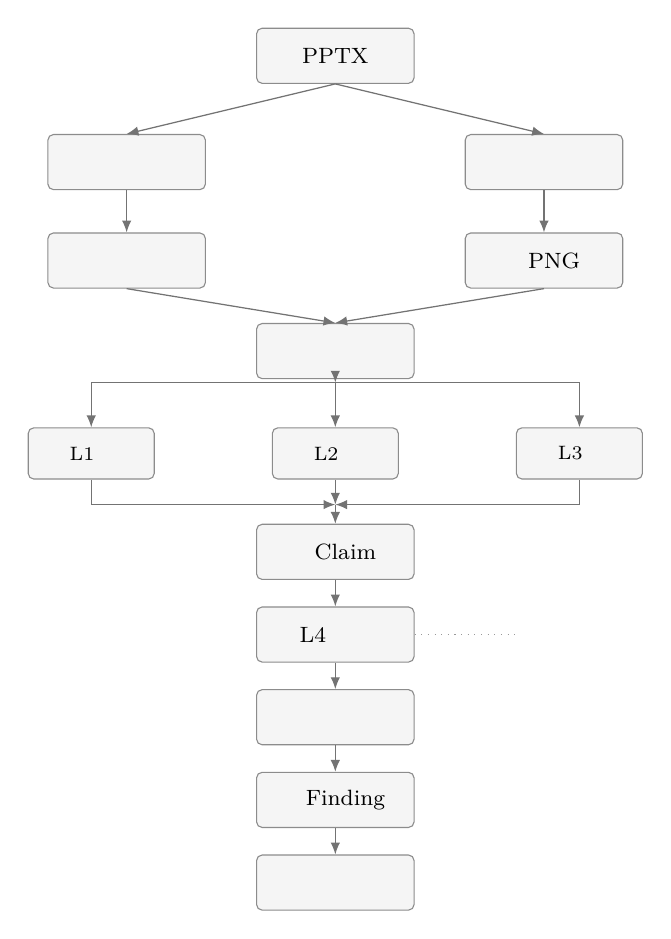
\begin{tikzpicture}[
  box/.style={draw=black!45, rounded corners=2pt, fill=black!4, align=center,
              font=\footnotesize, inner sep=3.5pt, minimum height=7mm, minimum width=20mm},
  leaf/.style={draw=black!45, rounded corners=2pt, fill=black!4, align=center,
              font=\scriptsize, inner sep=3pt, minimum height=6.5mm, minimum width=16mm},
  ar/.style={-{Latex[length=1.5mm,width=1.2mm]}, draw=black!55, line width=0.45pt}
]
\node[box] (pptx)   at (5.0,  0.00) {PPTX};
\node[box] (parse)  at (2.35, -1.35) {结构解析};
\node[box] (render) at (7.65, -1.35) {页面渲染};
\node[box] (elem)   at (2.35, -2.60) {元素表};
\node[box] (png)    at (7.65, -2.60) {逐页 PNG};
\node[box] (feat)   at (5.00, -3.75) {特征表};

\node[leaf] (l1) at (1.90, -5.05) {L1 规则};
\node[leaf] (l2) at (5.00, -5.05) {L2 视觉};
\node[leaf] (l3) at (8.10, -5.05) {L3 风格};

\node[box] (claim)   at (5.0, -6.30) {判决 Claim};
\node[box] (l4)      at (5.0, -7.35) {L4 语义（按需）};
\node[box] (fuse)    at (5.0, -8.40) {融合与按需复核};
\node[box] (finding) at (5.0, -9.45) {结论 Finding};
\node[box] (report)  at (5.0, -10.50) {审查报告};

\draw[ar] (pptx.south) -- (parse.north);
\draw[ar] (pptx.south) -- (render.north);
\draw[ar] (parse) -- (elem);
\draw[ar] (render) -- (png);
\draw[ar] (elem.south) -- (feat.north);
\draw[ar] (png.south) -- (feat.north);

\coordinate (bus)  at (5.0, -4.15);
\coordinate (bus2) at (5.0, -5.70);
\draw[ar] (feat.south) -- (bus);
\draw[ar] (bus) -- (l2.north);
\draw[ar] (bus) -| (l1.north);
\draw[ar] (bus) -| (l3.north);

\draw[ar] (l2.south) -- (bus2);
\draw[ar] (l1.south) |- (bus2);
\draw[ar] (l3.south) |- (bus2);
\draw[ar] (bus2) -- (claim.north);

\draw[ar] (claim) -- (l4);
\draw[ar] (l4) -- (fuse);
\draw[ar] (fuse) -- (finding);
\draw[ar] (finding) -- (report);

\node[font=\scriptsize, text=black!55, anchor=west] (need) at (7.30, -7.35) {仅按需调用};
\draw[dotted, draw=black!40, line width=0.4pt] (l4.east) -- (need.west);
\end{tikzpicture}
\end{center}

关键点：所有检测器\textbf{先输出''判决''而非''结论''}。判决包含''存在''与''不存在''两种取值，只有''存在''的判决在融合后转为结论。这样做的原因见
4.6 节。

\subsection{3.3
可独立运行的模块原则}\label{ux53efux72ecux7acbux8fd0ux884cux7684ux6a21ux5757ux539fux5219}

各检测模块互不依赖，任一模块失效不影响其余模块出结论。这条原则的工程意义在于：即使分类器性能不理想、参考资料检索未完成，基础审查与按需复核流程仍可完整演示。它同时是开发路线的组织依据（见第
7 节）。

\section{4 关键方法}\label{ux5173ux952eux65b9ux6cd5}

\subsection{4.1
缺陷体系与证据族}\label{ux7f3aux9677ux4f53ux7cfbux4e0eux8bc1ux636eux65cf}

缺陷按\textbf{现象族}分为四类，命名前缀供报告组织与用户阅读使用：

{\def\LTcaptype{none} % do not increment counter
\begin{longtable}[]{@{}llll@{}}
\toprule\noalign{}
前缀 & 族 & 判定所需的最小证据 & 典型检测层 \\
\midrule\noalign{}
\endhead
\bottomrule\noalign{}
\endlastfoot
S- & 结构 & PPTX 对象的几何、属性、层级关系 & L1 \\
V- & 视觉 & 页面渲染图像的统计特征 & L2 \\
M- & 语义 & 文本含义、图文关系、跨页逻辑 & L4 \\
R- & 要求 & 用户原始要求或参考资料与结果的比对 & L4 \\
\end{longtable}
}

\textbf{编码前缀表达''这是什么问题''，不表达''该由谁检测''。}
二者通常一致，但允许例外：例如''视觉层次弱''属视觉现象，但其最小证据是字号属性，不需要渲染图，因此路由到
L1。这条解耦规则避免了实现阶段用 \texttt{code{[}0{]}}
推断路由所带来的隐性错误。

\subsection{4.2 检测路由}\label{ux68c0ux6d4bux8defux7531}

路由由缺陷类别表显式给定，不由前缀推断。下表为首批实现的缺陷：

{\def\LTcaptype{none} % do not increment counter
\begin{longtable}[]{@{}lllll@{}}
\toprule\noalign{}
编码 & 名称 & 族 & 首选层 & 批次 \\
\midrule\noalign{}
\endhead
\bottomrule\noalign{}
\endlastfoot
S-OVERSHOOT & 元素越界 & S & L1 & 首批 \\
S-TEXT-OVERFLOW & 文字溢出 & S & L1 & 首批 \\
S-FONT-FALLBACK & 字体替换 & S & L1 & 首批 \\
S-PAGECOUNT & 页数超限 & S & L1 & 首批 \\
S-DECO-COUNT & 装饰元素过量 & S & L1 & 首批 \\
V-WHITESPACE & 留白失衡 & V & L2 & 首批 \\
V-TEMPLATE-REPEAT & 布局模板化 & V & L2 & 首批 \\
V-HIERARCHY & 视觉层次弱 & V & \textbf{L1} & 二批 \\
M-CROSSPAGE & 跨页不一致 & M & L4 & 首批 \\
R-CONTENT-MISS & 要求内容缺失 & R & L4 & 首批 \\
\end{longtable}
}

这张表同时是成本论证的骨架：结构族占比越高，``全部交给大模型''越不经济。该比例需在真实样本上统计，不得先验假定。

\subsection{4.3
PTPS：单页模板化特征分}\label{ptpsux5355ux9875ux6a21ux677fux5316ux7279ux5f81ux5206}

PTPS（Per-slide Template Pattern
Score）衡量\textbf{单页}在多大程度上呈现模板化生产特征，取值 0 至
100，越高越模板化。

\[\mathrm{PTPS} = 100 \times (0.4A + 0.3T + 0.3D)\]

{\def\LTcaptype{none} % do not increment counter
\begin{longtable}[]{@{}
  >{\raggedright\arraybackslash}p{(\linewidth - 4\tabcolsep) * \real{0.1607}}
  >{\raggedright\arraybackslash}p{(\linewidth - 4\tabcolsep) * \real{0.3929}}
  >{\raggedright\arraybackslash}p{(\linewidth - 4\tabcolsep) * \real{0.4464}}@{}}
\toprule\noalign{}
\begin{minipage}[b]{\linewidth}\raggedright
分项
\end{minipage} & \begin{minipage}[b]{\linewidth}\raggedright
含义
\end{minipage} & \begin{minipage}[b]{\linewidth}\raggedright
计算
\end{minipage} \\
\midrule\noalign{}
\endhead
\bottomrule\noalign{}
\endlastfoot
A 对齐规整度 & 元素边缘落在 12 列栅格上的比例 & 对齐元素数 ÷ 元素总数 \\
T 类型单调度 & 元素类型分布的集中程度 & \(1 - H(p)/\log K\)，\(H\)
为类型分布熵 \\
D 装饰密度 & 装饰性元素占比 & 装饰元素数 ÷ 元素总数 \\
\end{longtable}
}

``装饰性元素''的操作定义需要前置说明，否则不可复现：满足以下任一条件的形状计为装饰------无文本内容、面积占比小于
0.5\%、形状类型为基本图形或图标且不承载数据。该定义是工程口径，须在报告中标注，并允许按场景调整。

\subsubsection{4.3.1
分数的语义边界}\label{ux5206ux6570ux7684ux8bedux4e49ux8fb9ux754c}

PTPS 高分既不表示''质量差''，也不表示''由 AI
生成''。这一点必须在定义处写死，否则指标会被误读。

\textbf{指标测的是结构规律性，不是设计质量。}
规范的企业品牌模板、咨询公司模板、学术会议模板，恰恰以栅格统一、版式类型少、留白规整为设计目标，因此会同时得到高
PTPS。这不是误判，而是定义使然------若把这类文件判为''有缺陷''，错的是判据，不是模板。

由此产生三条实现约束：

\begin{enumerate}
\def\labelenumi{\arabic{enumi}.}
\tightlist
\item
  \textbf{PTPS 与 HCI 不进入风险等级，不作为 Finding 的一种。}
  它们与结论清单并列展示，属描述性指标，不参与''先改哪一页''的排序。
\item
  \textbf{不触发按需复核。}
  复核的对象是''某条结论是否成立''，而不是''某个分数是否偏高''；对指标本身再问一次模型，只会得到一句无依据的附和。
\item
  \textbf{界面只写''结构规律性''，不写''AI 味''。}
  同一屏内固定给出一句说明：模板化程度高不等于质量差，规范的品牌模板同样会得高分。
\end{enumerate}

指标本身的效度可用一个廉价检查代替：若定义成立，企业模板与 AI
生成稿应同时落在高分区，而杂志式排版、手绘风格的稿件应显著更低。若三类样本的分布无法区分，说明分项只测到了''元素多少''，需要重设而非调参。

\subsection{4.4
HCI：整份同质化指数}\label{hciux6574ux4efdux540cux8d28ux5316ux6307ux6570}

HCI（Homogeneity and Cliché
Index）衡量\textbf{整份文稿内部}的重复程度，取值 0 至 100。

\[\mathrm{HCI} = 100 \times (0.5R_{\text{adj}} + 0.3R_{\text{global}} + 0.2(1 - V_{\text{type}}))\]

{\def\LTcaptype{none} % do not increment counter
\begin{longtable}[]{@{}
  >{\raggedright\arraybackslash}p{(\linewidth - 4\tabcolsep) * \real{0.3036}}
  >{\raggedright\arraybackslash}p{(\linewidth - 4\tabcolsep) * \real{0.4464}}
  >{\raggedright\arraybackslash}p{(\linewidth - 4\tabcolsep) * \real{0.2500}}@{}}
\toprule\noalign{}
\begin{minipage}[b]{\linewidth}\raggedright
分项
\end{minipage} & \begin{minipage}[b]{\linewidth}\raggedright
含义
\end{minipage} & \begin{minipage}[b]{\linewidth}\raggedright
计算
\end{minipage} \\
\midrule\noalign{}
\endhead
\bottomrule\noalign{}
\endlastfoot
\(R_{\text{adj}}\) 相邻重复 & 相邻页布局特征余弦相似度超阈值的页对比例 &
超阈页对数 ÷ 相邻页对数 \\
\(R_{\text{global}}\) 全局重复 & 任意两页超阈相似的比例 & 超阈页对数 ÷
全部页对数 \\
\(V_{\text{type}}\) 版式多样性 & 不同版式的数量占比 & 版式簇数 ÷ 页数 \\
\end{longtable}
}

计算前置条件为页数不少于 8。少于 8
页不计算，因为页间重复需要足够的页对才能成立；这是硬约束而非保守设定。

阈值（相似度
0.92）、权重（0.5/0.3/0.2）与归一化参数均为工程默认值，未经数据校准，报告中须标注。

\subsection{4.5 PTPS 与 HCI
的分工}\label{ptps-ux4e0e-hci-ux7684ux5206ux5de5}

两个指标容易混淆，必须在定义上分开，否则会重复计数同一现象。

\textbf{PTPS 回答''这一页像不像模板做出来的''，HCI
回答''整份是不是同一个模板反复用''。}
前者是页内量，后者是页间量，二者可以独立变化：

{\def\LTcaptype{none} % do not increment counter
\begin{longtable}[]{@{}llll@{}}
\toprule\noalign{}
情形 & PTPS & HCI & 解释 \\
\midrule\noalign{}
\endhead
\bottomrule\noalign{}
\endlastfoot
每页都精工细作但版式相同 & 低 & 高 & 单页质量好，整份单调 \\
单页随手堆砌但每页都不同 & 低 & 低 & 谈不上模板化，只是粗糙 \\
单页高度规整但版式各异 & 高 & 低 & 模板化生产，但选了多种版式 \\
单页规整且版式一致 & 高 & 高 & 典型的批量生成特征 \\
\end{longtable}
}

按此划分，PTPS 的三个分项均为页内量，HCI
的三个分项均为页间量，不存在重叠。这一划分相对前期文档做了收窄：装饰密度归入
PTPS，HCI 不再包含页内项。

\textbf{两个指标既不构成来源判定，也不构成质量判定。}

\begin{itemize}
\tightlist
\item
  不构成来源判定：人工制作的模板同样可以得到高分。指标衡量的是作品自身的结构规律性，不是作者的归属。
\item
  不构成质量判定：规范的品牌模板以统一栅格与稳定版式为设计目标，会同时得到高
  PTPS 与高 HCI，但它属于好设计。若把它读成''缺陷''，错在判据。
\item
  因此二者只作描述性呈现，不进入风险分级，也不进入按需复核的触发条件（理由见
  4.3.1）。
\end{itemize}

\subsection{4.6
判决与结论分离：为什么需要两层}\label{ux5224ux51b3ux4e0eux7ed3ux8bbaux5206ux79bbux4e3aux4ec0ux4e48ux9700ux8981ux4e24ux5c42}

所有检测器先输出 \texttt{Claim}（判决），再由融合层生成
\texttt{Finding}（结论）。这一层看似多余，实则不可或缺：

\textbf{其一，冲突检测需要''否定''这一侧。}
若检测器只记录''发现了什么''，那么''规则判定越界、视觉模型判定不存在''这句最关键的分歧永远无法表达------因为其中的''不存在''没有地方存放。有了判决层，冲突可以被显式记录，并直接驱动降级为''待人工核实''。

\textbf{其二，覆盖率统计需要它。}
回答''某方案在哪些缺陷类别上做了有效判断''时，需要知道某检测器在该类别上是否给出了判断（无论正负）。只记录正例，覆盖率无法计算，实验二的方案对比也就失去了可比性。

融合后的结论携带以下核心字段：页码、缺陷编码、严重度、状态、置信度及其来源、证据引用、解释、建议、成本与检测器清单。

\textbf{严重度与状态必须正交。}
严重度回答''多要紧''，状态回答''多确定''。``高严重度 +
待核实''是完全合法的组合，且恰恰是最需要提醒用户的情形：报出来，但明确说明证据不足。

\subsection{4.7
按需复核：系统中唯一的自主决策}\label{ux6309ux9700ux590dux6838ux7cfbux7edfux4e2dux552fux4e00ux7684ux81eaux4e3bux51b3ux7b56}

这是全系统唯一一处真正意义上的''决策''，也是''智能体''三个字唯一站得住的地方。

\subsubsection{4.7.1
三种置信度不是同一种量}\label{ux4e09ux79cdux7f6eux4fe1ux5ea6ux4e0dux662fux540cux4e00ux79cdux91cf}

实现这条决策最容易犯的错，是给所有检测器设同一条阈值。三种来源的
\texttt{confidence} 在数学性质上完全不同，直接比较会得到系统性偏差：

{\def\LTcaptype{none} % do not increment counter
\begin{longtable}[]{@{}
  >{\raggedright\arraybackslash}p{(\linewidth - 6\tabcolsep) * \real{0.1475}}
  >{\raggedright\arraybackslash}p{(\linewidth - 6\tabcolsep) * \real{0.2623}}
  >{\raggedright\arraybackslash}p{(\linewidth - 6\tabcolsep) * \real{0.1475}}
  >{\raggedright\arraybackslash}p{(\linewidth - 6\tabcolsep) * \real{0.4426}}@{}}
\toprule\noalign{}
\begin{minipage}[b]{\linewidth}\raggedright
来源
\end{minipage} & \begin{minipage}[b]{\linewidth}\raggedright
输出形态
\end{minipage} & \begin{minipage}[b]{\linewidth}\raggedright
可否作概率
\end{minipage} & \begin{minipage}[b]{\linewidth}\raggedright
正确处理
\end{minipage} \\
\midrule\noalign{}
\endhead
\bottomrule\noalign{}
\endlastfoot
规则 & 布尔值 + 物理裕度（超出边界多少 pt） & 否 & 裕度接近 0
时视为边界情形，其余直接确定 \\
分类器 & 概率（未校准） & 校准后可 & 先做 Platt 或 isotonic 校准
{[}6{]}，用校准后概率设带，并给出可靠性图 \\
大模型自评 & 序数标签（高 / 中 / 低） & 不能 &
只取''低''\,``中''触发复核，不与分类器概率比较 \\
\end{longtable}
}

两个具体理由。其一，分类器的原始输出不是概率------SVM
的决策值可落在任意区间，即便逻辑回归的输出也常偏离真实频率，未经校准直接阈值化会系统性偏高或偏低；现代网络的过度自信已被系统验证
{[}7{]}。其二，大模型的自评置信度是语言判断而非概率，把它与 0.47
这样的数值比大小，等于把两种量纲混为一谈。

融合层的做法是：\textbf{同源内部比较数值，跨源只比较序数。}
各来源先映射到''确定 / 可能 /
待核实''三档，取最保守者；不拿模型概率与''中等置信''直接比大小。

\subsubsection{4.7.2 触发条件}\label{ux89e6ux53d1ux6761ux4ef6}

{\def\LTcaptype{none} % do not increment counter
\begin{longtable}[]{@{}
  >{\raggedright\arraybackslash}p{(\linewidth - 4\tabcolsep) * \real{0.4932}}
  >{\raggedright\arraybackslash}p{(\linewidth - 4\tabcolsep) * \real{0.2055}}
  >{\raggedright\arraybackslash}p{(\linewidth - 4\tabcolsep) * \real{0.3014}}@{}}
\toprule\noalign{}
\begin{minipage}[b]{\linewidth}\raggedright
触发条件
\end{minipage} & \begin{minipage}[b]{\linewidth}\raggedright
判定依据
\end{minipage} & \begin{minipage}[b]{\linewidth}\raggedright
处理
\end{minipage} \\
\midrule\noalign{}
\endhead
\bottomrule\noalign{}
\endlastfoot
两个检测器结论相反 & verdict 冲突 & 追加一次大模型复核 \\
分类器校准后概率落入 0.5±0.1 & 校准概率 & 追加一次复核 \\
大模型自评置信为''低''或''中'' & 序数标签 & 追加一次复核 \\
缺陷为最高严重度但仅单源支持 & 来源计数 = 1 & 追加一次复核 \\
要求类缺陷但用户未提供要求 & 缺输入 & 不追加，直接标记待核实 \\
\end{longtable}
}

带的具体数值（0.5±0.1）是初始工程默认值，须写进代码常量表并在报告附录列出。\textbf{阈值的调整只允许在验证集上做，不允许在测试集上回调}------否则实验三的''人工复核条数''会被阈值调优污染。

复核次数、复核命中率（复核后结论被改变的比例）与因此节省的调用数必须计数并纳入报告。否则''分层省钱''只是一句宣称。

其余环节的''调度''本质是查表：编码确定，路径即确定。项目不将这部分包装为自主规划。

\subsection{4.8
三级可执行建议}\label{ux4e09ux7ea7ux53efux6267ux884cux5efaux8bae}

``建议优化排版''不是可执行建议。本项目将建议分为三级，结构类缺陷要求达到第三级：

\begin{itemize}
\tightlist
\item
  \textbf{L1 定位}：哪一页、哪个对象。例：第 7 页右侧第二个文本框。
\item
  \textbf{L2 数值}：改什么、改成多少。例：框宽 9.2 cm，可用 8.4
  cm，建议缩至 8.2 cm。
\item
  \textbf{L3 操作}：在软件中如何操作。例：设置形状格式 → 文本选项 →
  关闭''自动调整''。
\end{itemize}

实现方式是一张 \texttt{缺陷编码\ →\ 建议模板}
的映射表，模板中带实测值占位符。这张表同时在项目中承担知识库角色：缺陷类型、所需证据、适用建议三者构成类---属性---关系结构，可序列化为
JSON，必要时转为 RDF。

\section{5
数据与模型方案}\label{ux6570ux636eux4e0eux6a21ux578bux65b9ux6848}

\subsection{5.1 SlideAudit
的构成与划分}\label{slideaudit-ux7684ux6784ux6210ux4e0eux5212ux5206}

SlideAudit 提供约 2,400
张带标注幻灯片图像，其构成需要在使用前核查：初步了解为约 600
张原始页面与约 1,800 个合成变体，即每个原始页面存在数个修改版本。

由此产生一条不可省略的划分要求：\textbf{按原始页面分组后再划分训练集与测试集}。若按单张图像随机划分，同一原图的不同变体将跨越两集，模型可能学到''改图痕迹''而非缺陷特征，全部指标随之失真。这一条必须在报告中写明。

另需注意：该数据集的元素坐标为图像检测所得，非 PPTX
原生结构。因此它只能支撑视觉层实验，不能用于验证规则层。

\subsection{5.2
特征方案：几何与视觉混合}\label{ux7279ux5f81ux65b9ux6848ux51e0ux4f55ux4e0eux89c6ux89c9ux6df7ux5408}

初期候选三类缺陷作为监督学习对象：留白分布不均、布局拥挤、字号使用不当。三类能否都成立，不取决于命名，而取决于特征能否从数据集里取出来------这是
5.3
节要裁定的事。先训练、再解释指标为何反常，是这类实验最常见的失败方式。

特征设计上有一项需要预先说明的技术判断：

\begin{quote}
\textbf{CLIP {[}5{]} 特征不适合单独承担几何类缺陷的判定。} CLIP
的预训练目标是图文对齐，其表征偏向语义与风格，对元素间距、越界、面积占比等精确空间关系不敏感。以
CLIP 特征单独训练''布局拥挤''分类器，性能很可能低于简单几何统计量。
\end{quote}

因此本项目采用\textbf{几何特征与 CLIP
特征拼接}的方案，并保留三组消融对比：

{\def\LTcaptype{none} % do not increment counter
\begin{longtable}[]{@{}
  >{\raggedright\arraybackslash}p{(\linewidth - 4\tabcolsep) * \real{0.1228}}
  >{\raggedright\arraybackslash}p{(\linewidth - 4\tabcolsep) * \real{0.6140}}
  >{\raggedright\arraybackslash}p{(\linewidth - 4\tabcolsep) * \real{0.2632}}@{}}
\toprule\noalign{}
\begin{minipage}[b]{\linewidth}\raggedright
特征组
\end{minipage} & \begin{minipage}[b]{\linewidth}\raggedright
内容
\end{minipage} & \begin{minipage}[b]{\linewidth}\raggedright
用途
\end{minipage} \\
\midrule\noalign{}
\endhead
\bottomrule\noalign{}
\endlastfoot
G 几何 & 元素数、覆盖率、留白四边占比、间距方差、字号分布 &
直接对应排版属性 \\
C 视觉 & CLIP 图像嵌入（降维后） & 捕捉整体观感与风格 \\
G+C 拼接 & 两组拼接 & 主方案 \\
\end{longtable}
}

消融结果本身即是一项可报告的结论：哪一类缺陷更依赖几何证据、哪一类更依赖视觉表征。这比单纯报告一个
F1 更有信息量。

\subsection{5.3
特征可提取性核查（训练前置）}\label{ux7279ux5f81ux53efux63d0ux53d6ux6027ux6838ux67e5ux8badux7ec3ux524dux7f6e}

一条硬性前置：\textbf{先证明特征能取出来，再谈训练。} SlideAudit
提供的是渲染图与图像检测得到的元素描述，不是 PPTX
结构，两者能供给的特征并不相同。

首要动作是把 \texttt{data/descriptions/}
的字段打印一遍。按仓库说明，每个元素只有三类信息：\texttt{type}、\texttt{positionAndSize.normalized}、\texttt{textContent}（或图像元信息）。据此逐项核对：

{\def\LTcaptype{none} % do not increment counter
\begin{longtable}[]{@{}
  >{\raggedright\arraybackslash}p{(\linewidth - 4\tabcolsep) * \real{0.2222}}
  >{\raggedright\arraybackslash}p{(\linewidth - 4\tabcolsep) * \real{0.1528}}
  >{\raggedright\arraybackslash}p{(\linewidth - 4\tabcolsep) * \real{0.6250}}@{}}
\toprule\noalign{}
\begin{minipage}[b]{\linewidth}\raggedright
计划特征
\end{minipage} & \begin{minipage}[b]{\linewidth}\raggedright
可得性
\end{minipage} & \begin{minipage}[b]{\linewidth}\raggedright
依据 / 替代方案
\end{minipage} \\
\midrule\noalign{}
\endhead
\bottomrule\noalign{}
\endlastfoot
元素数 & 可直接提取 & \texttt{elements} 列表长度 \\
元素覆盖率 & 可直接提取 & 各 bbox 的 width×height
求和（重叠区会重复计入，须先合并） \\
留白四边占比 & 可直接提取 & bbox 到画布四边的距离，分边统计 \\
间距方差 & 可直接提取 & 元素两两间距的分布 \\
类型分布 / 类型单调度 & 可直接提取 & \texttt{type} 字段 \\
栅格对齐度 & 近似可得 & 由 bbox 边缘坐标聚类估计，非真实栅格 \\
\textbf{字号分布} & \textbf{不可得} &
描述中无字号字段；仅能由文本行高像素反推，误差不可控 \\
\end{longtable}
}

由此得到三条结论，需在实验开始前落定：

\textbf{其一，``字号使用不当''应移出实验一。}
该类别的最小证据是字号属性，图像侧无法可靠还原；而它在本项目中本就由
\texttt{V-HIERARCHY} 以''标题字号 ÷
正文字号''的规则形式呈现------规则不需要训练。硬把它塞进监督学习，只会得到一个无法解释的
F1。

\textbf{其二，实验一的类别数由 3 收缩为 2。}
留白失衡与布局拥挤均可由上述几何特征支撑。若核查发现这两类在特征空间上高度重叠（例如留白占比在正负类上的分布几乎重合），则再降一级：不与
SVM 对比，只报告阈值法与逻辑回归，并说明原因。

\textbf{其三，标签质量也要先查。} 每条标注带
\texttt{has\_strong\_agreement}
字段，训练与评测应只用强一致样本；弱一致样本单列，用作''标注噪声对指标影响''的分析材料，而不是直接丢弃。\texttt{metadata/slideaudit\_metadata.csv}
中的 \texttt{source\_type}
可用于检查来源分布，避免训练集与测试集的来源系统性偏斜。

这一步的产出是一张核查表（特征 × 可得性 ×
替代方案），在阶段一结束前完成。\textbf{核查不过就换特征或换类别，不允许训完再解释指标为何反常。}

\subsection{5.4
分类器与对照}\label{ux5206ux7c7bux5668ux4e0eux5bf9ux7167}

{\def\LTcaptype{none} % do not increment counter
\begin{longtable}[]{@{}ll@{}}
\toprule\noalign{}
方案 & 说明 \\
\midrule\noalign{}
\endhead
\bottomrule\noalign{}
\endlastfoot
阈值法 & 对每个几何指标设定阈值，作为下界基线 \\
逻辑回归 & 主方案；多标签采用各类独立判定 \\
SVM & 对照方案，核函数取 RBF \\
\end{longtable}
}

多标签采用一类一模型的独立二分类，而非单一
softmax。评估按类别计算精确率、召回率与 F1，并给出宏平均与微平均。

\subsection{5.5 自建评测集}\label{ux81eaux5efaux8bc4ux6d4bux96c6}

训练数据来自公开数据集，评测数据必须自建，因为需要配套的原始要求与参考资料。

规模分两档，第一版不追 30 份：

{\def\LTcaptype{none} % do not increment counter
\begin{longtable}[]{@{}
  >{\raggedright\arraybackslash}p{(\linewidth - 6\tabcolsep) * \real{0.2000}}
  >{\raggedright\arraybackslash}p{(\linewidth - 6\tabcolsep) * \real{0.1857}}
  >{\raggedright\arraybackslash}p{(\linewidth - 6\tabcolsep) * \real{0.1714}}
  >{\raggedright\arraybackslash}p{(\linewidth - 6\tabcolsep) * \real{0.4429}}@{}}
\toprule\noalign{}
\begin{minipage}[b]{\linewidth}\raggedright
项
\end{minipage} & \begin{minipage}[b]{\linewidth}\raggedright
第一版
\end{minipage} & \begin{minipage}[b]{\linewidth}\raggedright
扩至
\end{minipage} & \begin{minipage}[b]{\linewidth}\raggedright
说明
\end{minipage} \\
\midrule\noalign{}
\endhead
\bottomrule\noalign{}
\endlastfoot
总数 & 12 份 / 180 页 & 20 份 / 300 页 & 30 份 / 450 页为上限，非目标 \\
真实 AI 生成 & 4 份 & 7 份 & 覆盖至少 3 个生成工具，保留原始提示词 \\
人工模板/课件 & 5 份 & 8 份 & 提供风格对照 \\
质量尚可的样本 & 3 份 & 5 份 & \textbf{负样本，用于计算误报率} \\
\end{longtable}
}

按此收缩的理由有三条：

\begin{enumerate}
\def\labelenumi{\arabic{enumi}.}
\tightlist
\item
  \textbf{标注成本按页线性增长，统计收益不是。} 180
  页已能给分类别点估计；再加 12
  份带来的置信区间收窄，与投入的十余小时不成比例。
\item
  \textbf{时间应投在两处回报更高的地方}：每份的盲标抽页（估计漏报），以及负样本比例。前者决定漏报率是否可信，后者决定误报率是否有分母，两者都比多标
  12 份要紧。
\item
  \textbf{缩规模时的取舍顺序固定}：先砍份数，不砍每份页数，不砍负样本比例。若砍到某类缺陷的正例进入个位数，该类退出实验二，只做描述性报告。
\end{enumerate}

第三类容易被忽略：若全部挑选''问题明显''的文件，系统报错时也无法被发现，误报率没有分母。此外，样本须为\textbf{可编辑对象}，即每页含多个可解析形状，而非一页一张图片------图片式文件会使结构证据整体归零。

人工标注只针对三类实验区缺陷，标注单元为''页面 + 区域 +
缺陷类型''，分三步完成：先判定存在性（是/否/不确定），再判定严重度，最后记录定位。存在性的一致率通常显著高于严重度，先冻结前者可避免两个维度互相污染。

标注采用机器初筛加人工裁决的方式：先由检测器输出候选问题列表，人工只做确认、否决与补充；同时每份随机抽取两页进行盲标（不看系统输出），用于估计漏报。这既节省时间，也避免了只看到系统已报问题的确认偏差。

\subsection{5.6
指标与成本口径}\label{ux6307ux6807ux4e0eux6210ux672cux53e3ux5f84}

{\def\LTcaptype{none} % do not increment counter
\begin{longtable}[]{@{}
  >{\raggedright\arraybackslash}p{(\linewidth - 6\tabcolsep) * \real{0.1607}}
  >{\raggedright\arraybackslash}p{(\linewidth - 6\tabcolsep) * \real{0.2857}}
  >{\raggedright\arraybackslash}p{(\linewidth - 6\tabcolsep) * \real{0.3036}}
  >{\raggedright\arraybackslash}p{(\linewidth - 6\tabcolsep) * \real{0.2500}}@{}}
\toprule\noalign{}
\begin{minipage}[b]{\linewidth}\raggedright
实验
\end{minipage} & \begin{minipage}[b]{\linewidth}\raggedright
对比对象
\end{minipage} & \begin{minipage}[b]{\linewidth}\raggedright
主指标
\end{minipage} & \begin{minipage}[b]{\linewidth}\raggedright
次指标
\end{minipage} \\
\midrule\noalign{}
\endhead
\bottomrule\noalign{}
\endlastfoot
一 分类可行性 & 阈值 / 逻辑回归 / SVM & 分类别 F1、PR 曲线 &
训练与推理耗时 \\
二 分层对比 & 仅规则 / 仅 ML / 分层协同 & 分类别 F1 &
\textbf{调用次数、token、耗时} \\
三 证据约束 & 直接问模型 / 证据约束 & 定位命中率、无依据断言比例 &
人工复核条数 \\
\end{longtable}
}

实验二有一条必须先解决的方法论问题：三类方案覆盖的缺陷类别不同，若在同一测试集上计算总体
F1，分层方案几乎必然最高，但胜出的原因只是覆盖面更广，而非方法更优。这属于覆盖度混淆。

处理办法是：主对比只放在\textbf{各方案都声称能检的公共类别}上（留白失衡既可写成阈值规则，也可由几何特征分类器判定，是最合适的对照点）；其余类别以''方案
×
类别''矩阵报告覆盖能力；成本与效果按同一单位计算，最后以曲线而非单一数字呈现。

成本口径须固定：调用次数按页计，token
只计输入与输出、不计缓存，规则层记为 0 次调用但注明其开发成本未计入。

\section{6 课程知识映射}\label{ux8bfeux7a0bux77e5ux8bc6ux6620ux5c04}

{\def\LTcaptype{none} % do not increment counter
\begin{longtable}[]{@{}
  >{\raggedright\arraybackslash}p{(\linewidth - 6\tabcolsep) * \real{0.1607}}
  >{\raggedright\arraybackslash}p{(\linewidth - 6\tabcolsep) * \real{0.4107}}
  >{\raggedright\arraybackslash}p{(\linewidth - 6\tabcolsep) * \real{0.2679}}
  >{\raggedright\arraybackslash}p{(\linewidth - 6\tabcolsep) * \real{0.1607}}@{}}
\toprule\noalign{}
\begin{minipage}[b]{\linewidth}\raggedright
课程内容
\end{minipage} & \begin{minipage}[b]{\linewidth}\raggedright
项目中的落点
\end{minipage} & \begin{minipage}[b]{\linewidth}\raggedright
对应产出
\end{minipage} & \begin{minipage}[b]{\linewidth}\raggedright
是否核心
\end{minipage} \\
\midrule\noalign{}
\endhead
\bottomrule\noalign{}
\endlastfoot
逻辑回归 & 视觉缺陷多标签分类 & 实验一主模型 & 是 \\
SVM & 与逻辑回归的分类效果对照 & 实验一对照组 & 是 \\
数据可视化 & 问题分布、执行过程、成本---效果曲线 & 报告图表与界面 &
是 \\
本体知识建模 & 缺陷编码、证据关系、建议知识库 & 建议模板库、缺陷类别表 &
是 \\
向量 RAG & 参考资料检索与基于证据的追问 & 完整性核验、追问 & 可降级 \\
智能体设计 & 工具编排、按需复核、状态管理 & 调度层 & 是 \\
\end{longtable}
}

知识建模一项容易被做成形式主义，本项目的落点尽量具体：缺陷类别表的每一行本身就是一个类，其''首选层''\,``所需证据''``建议模板''是属性，而''某缺陷需要哪类证据''\,``某证据支持哪些缺陷''构成关系。报告生成时按图查询建议，而不是写一长串
\texttt{if} 分支。

RAG
一项属于可降级模块：参考资料覆盖检查可以在没有向量检索的情况下，用要素抽取加字符串匹配实现；向量检索主要改善''表述不同但含义相同''的召回。若时间不足，该模块降级不影响主链路。

\section{7 开发路线}\label{ux5f00ux53d1ux8defux7ebf}

五个阶段，每阶段结束时都有可演示的产物，且不依赖后续阶段。

{\def\LTcaptype{none} % do not increment counter
\begin{longtable}[]{@{}
  >{\raggedright\arraybackslash}p{(\linewidth - 6\tabcolsep) * \real{0.1731}}
  >{\raggedright\arraybackslash}p{(\linewidth - 6\tabcolsep) * \real{0.2500}}
  >{\raggedright\arraybackslash}p{(\linewidth - 6\tabcolsep) * \real{0.2885}}
  >{\raggedright\arraybackslash}p{(\linewidth - 6\tabcolsep) * \real{0.2885}}@{}}
\toprule\noalign{}
\begin{minipage}[b]{\linewidth}\raggedright
阶段
\end{minipage} & \begin{minipage}[b]{\linewidth}\raggedright
内容
\end{minipage} & \begin{minipage}[b]{\linewidth}\raggedright
阶段产物
\end{minipage} & \begin{minipage}[b]{\linewidth}\raggedright
通过判据
\end{minipage} \\
\midrule\noalign{}
\endhead
\bottomrule\noalign{}
\endlastfoot
一 基础审查 & PPTX 解析、页面渲染、越界与字号规则 & 可对任意 PPTX
输出带页码与对象信息的报告 & 5 份样本全部出图，坐标对齐误差小于 2 pt \\
二 智能体最小闭环 & 路由、冲突判定、按需复核、成本计数 &
一条能自己决定''要不要再查一次''的链路 &
复核可触发、可计数，冲突能正确降级 \\
三 机器学习 & 特征可提取性核查、数据整理、分类器训练 & 实验一结果与对照
& 分类器可运行，有分类别指标与 PR 曲线 \\
四 风格分析 & PTPS 与 HCI 计算、明细清单 & 分数、分项、证据页清单 &
两项指标可复算，明细可追溯到具体页面 \\
五 界面与报告 & Streamlit 界面、报告生成、追问 &
上传---审查---复核---报告的完整流程 & 端到端无人工干预跑通一份 PPT \\
\end{longtable}
}

\textbf{阶段顺序按依赖关系排，不按工作量排；交付优先级与阶段顺序是两件事。}
阶段二紧跟阶段一，是刻意的：智能体闭环只需要''一组规则结论 +
一次复核调用''，既不需要等分类器训好，也不需要等风格指标算完。若把整合排到最后，一旦时间不足，被砍掉的恰好是课程真正评分的那部分------决策链，而不是检测器数量。

最小闭环里的模型调用只承担一件事：对被判定为不确定或存在冲突的单条结论，给出''成立
/ 不成立 / 无法判断''三选一及一句理由，输出为固定三字段的
JSON。这比实现完整的跨页语义检测便宜一个数量级，却足以让''按需复核''真实成立。按此顺序推进，任意时刻中断，交付的仍是一个可演示的完整系统，差别只在覆盖面的宽窄：

\begin{itemize}
\tightlist
\item
  \textbf{阶段一结束}：纯规则的结构审查报告，零 API
  调用；但没有决策链，不体现智能体。
\item
  \textbf{阶段二结束}：检测 → 冲突 → 复核 → 降级 → 报告的完整链路，覆盖
  2--3 类缺陷；机器学习与风格指标缺位。
\item
  \textbf{阶段三结束}：上述链路加一个有独立测试结果的分类器；风格指标仍缺位。
\item
  \textbf{阶段四结束}：再加 PTPS / HCI 与明细；界面仍为命令行输出。
\item
  \textbf{阶段五结束}：完整系统。
\end{itemize}

\textbf{阶段二结束那一档是本项目的最低可交付线}：宁可只检三类但会自己复核，也不要检八类但只会罗列。这一条同时约束砍单顺序------时间不足时先砍阶段四，其次把阶段五降为静态
HTML 报告，阶段一与二不砍。

阶段一有一条前置判断必须在第一天完成：\textbf{抽 5 份
PPTX，统计每页的形状数量。}
若多数页面只有一个图片对象，说明文件为图片式导出，结构证据整体失效，须当天调整方案（改为以渲染图为主，或补充可编辑样本）。这一步只需十分钟，却决定后续所有假设是否成立。

渲染方案采用 \textbf{PowerPoint COM 优先、LibreOffice headless
备选}。前者保真度最高，尤其是中文字体与行距；后者用于交叉验证与环境迁移。需注意：同一份
PPTX
在两条管线下的字体回退与行距算法不同，会直接影响''文字溢出''与''留白失衡''的判定结果。因此标注所用的渲染图与检测所用的渲染图必须来自同一管线，否则测出的是渲染器差异而非文稿质量。

\section{8
风险与已知局限}\label{ux98ceux9669ux4e0eux5df2ux77e5ux5c40ux9650}

{\def\LTcaptype{none} % do not increment counter
\begin{longtable}[]{@{}
  >{\raggedright\arraybackslash}p{(\linewidth - 4\tabcolsep) * \real{0.2727}}
  >{\raggedright\arraybackslash}p{(\linewidth - 4\tabcolsep) * \real{0.3273}}
  >{\raggedright\arraybackslash}p{(\linewidth - 4\tabcolsep) * \real{0.4000}}@{}}
\toprule\noalign{}
\begin{minipage}[b]{\linewidth}\raggedright
风险
\end{minipage} & \begin{minipage}[b]{\linewidth}\raggedright
触发信号
\end{minipage} & \begin{minipage}[b]{\linewidth}\raggedright
应对
\end{minipage} \\
\midrule\noalign{}
\endhead
\bottomrule\noalign{}
\endlastfoot
样本为图片式 & 首日体检发现多数页面仅一个图片对象 &
补充可编辑样本；或将规则层改测渲染图可判的属性，重写假设 \\
渲染字体缺失 & 抽查出现方块字或字体替换 &
安装缺失字体；否则更换字体族并在报告中声明 \\
SlideAudit 标签不覆盖目标类别 & 标签清单无''留白''对应项 &
更换目标类别，或改用自建样本训练，结论降级 \\
SlideAudit 特征不可提取 & 核查表出现''不可得''项 &
该类移出实验一，改由规则或自建样本验证；不先训练再解释 \\
CLIP 对几何属性不敏感 & 消融显示仅视觉特征时 F1 显著低 &
已有应对：几何特征为主，视觉特征为辅；如实报告消融结果 \\
分类器效果不达预期 & 测试集 F1 低于 0.40 &
并列报告阈值法与分类器，结论写''在该特征集与样本量下，监督学习未显著优于阈值法'' \\
评测样本标注滞后 & 阶段三时完成度不足 12 份 & 按 5.5
节的第一版规模先跑，不缩减每份页数与负样本比例 \\
时间不足 & 阶段二结束仍未跑通闭环 & 按第 7
节的中断优先级：保一、二（决策链），砍四（风格指标），五退为静态 HTML
报告 \\
模型 API 不可用或限流 & 复核调用连续失败 & 复核降级为''标记待核实 +
记录失败次数''，不伪造结论，成本栏注明 \\
\end{longtable}
}

三条已知局限需要写在报告的显著位置，而非藏在附录：

\textbf{其一，样本量有限。} 第一版 12 份、约 180 页，视进度扩至 20
份、约 300
页。这足以支撑分类别的点估计与方案间排序，不足以支撑精细的置信区间；报告只给点估计并明确样本规模，不外推为普遍结论。

\textbf{其二，渲染管线的偏差未被完全消除。}
无论选择哪条管线，渲染结果与用户在 PowerPoint
中看到的画面都会存在差异，这部分差异无法从指标中分离。

\textbf{其三，PTPS 与 HCI 的阈值未校准。}
当前权重与阈值均为工程默认值，未经数据拟合。校准与否只影响分数高低，不影响''该指标可计算''这一事实------这与''AI
生成概率''有本质区别：后者缺少基线即不成立，前者缺少校准只是不精确。另需重申
4.3.1
的边界：分数只表示结构规律性，不表示设计质量，规范模板同样会得高分。

\section{9 预期成果}\label{ux9884ux671fux6210ux679c}

\subsection{9.1 系统层面}\label{ux7cfbux7edfux5c42ux9762}

一套可本地运行的审查系统，输入 PPTX
与可选的原始要求、参考资料，输出交互式审查报告，包含：按页问题清单、证据定位、风险分级、可执行建议、PTPS
与 HCI 分数及明细、以及本次审查的模型调用成本。

\subsection{9.2 实验层面}\label{ux5b9eux9a8cux5c42ux9762}

三组可复现的对照结果：分类可行性（阈值 / 逻辑回归 /
SVM，覆盖留白失衡与布局拥挤两类）、分层对比（仅规则 / 仅 ML /
分层协同，含成本）、证据约束（有 /
无证据绑定的结论质量）。以及特征消融结果（几何 / 视觉 / 拼接）。

\subsection{9.3 方法层面}\label{ux65b9ux6cd5ux5c42ux9762}

若实验支持，本项目可以给出一个可复用的判断：\textbf{在演示文稿质量审查中，不同缺陷类型的最优检测层不同，且这一差异可由证据可得性解释。}
若实验结果不支持，则如实报告负结果并分析原因------这同样是有效的结论。

\subsection{9.4 一句话}\label{ux4e00ux53e5ux8bdd}

\textbf{这个项目的下限由工程保证（渲染通即稳），上限由评测集的标注质量决定，第一印象由界面决定。三者不能互相替代。}

\section{参考文献}\label{ux53c2ux8003ux6587ux732e}

{[}1{]} Zhang Z, Chen R, Zhong M, Wobbrock J O. SlideAudit: A Dataset
and Taxonomy for Automated Evaluation of Presentation
Slides{[}C{]}//Proceedings of the 38th Annual ACM Symposium on User
Interface Software and Technology (UIST '25). ACM, 2025. DOI:
10.1145/3746059.3747736.

{[}2{]} Zheng H, Guan X, Kong H, Zheng J, Zhou W, Lin H, Lu Y, He B, Han
X, Sun L. PPTAgent: Generating and Evaluating Presentations Beyond
Text-to-Slides{[}J{]}. arXiv preprint arXiv:2501.03936, 2025.（PPTEval
评测框架随本文提出）

{[}3{]} Chen X-S, Zhu J, Li P, Wang H, Yang S, Guo M-H. PresentBench: A
Fine-Grained Rubric-Based Benchmark for Slide Generation{[}J{]}. arXiv
preprint arXiv:2603.07244, 2026.

{[}4{]} Lu Y, Knearem T, Dutta S, Blass J, Kliman-Silver C, Bentley F.
AI Is Not Enough: A Hybrid Technical Approach to AI Adoption in UI
Linting With Heuristics{[}C{]}//Extended Abstracts of the CHI Conference
on Human Factors in Computing Systems (CHI EA '24). ACM, 2024: Article
501. DOI: 10.1145/3613905.3637135.

{[}5{]} Radford A, Kim J W, Hallacy C, et al.~Learning Transferable
Visual Models From Natural Language Supervision{[}C{]}//Proceedings of
the 38th International Conference on Machine Learning (ICML). PMLR,
2021: 8748--8763.

{[}6{]} Platt J. Probabilistic Outputs for Support Vector Machines and
Comparisons to Regularized Likelihood Methods{[}M{]}//Advances in Large
Margin Classifiers. MIT Press, 1999: 61--74.

{[}7{]} Guo C, Pleiss G, Sun Y, Weinberger K Q. On Calibration of Modern
Neural Networks{[}C{]}//Proceedings of the 34th International Conference
on Machine Learning (ICML). PMLR, 2017: 1321--1330.

数据集与代码资源：

{[}8{]} SlideAudit 数据集与代码.
https://github.com/zhuohaouw/SlideAudit（CC BY 4.0）

{[}9{]} PresentBench 数据集.
https://huggingface.co/datasets/PresentBench/PresentBench（任务指令与
checklist 采用 CC BY-NC 4.0）

\section{附录 A
统一结论记录的核心字段}\label{ux9644ux5f55-a-ux7edfux4e00ux7ed3ux8bbaux8bb0ux5f55ux7684ux6838ux5fc3ux5b57ux6bb5}

{\def\LTcaptype{none} % do not increment counter
\begin{longtable}[]{@{}
  >{\raggedright\arraybackslash}p{(\linewidth - 4\tabcolsep) * \real{0.3750}}
  >{\raggedright\arraybackslash}p{(\linewidth - 4\tabcolsep) * \real{0.1250}}
  >{\raggedright\arraybackslash}p{(\linewidth - 4\tabcolsep) * \real{0.5000}}@{}}
\toprule\noalign{}
\begin{minipage}[b]{\linewidth}\raggedright
字段
\end{minipage} & \begin{minipage}[b]{\linewidth}\raggedright
类型
\end{minipage} & \begin{minipage}[b]{\linewidth}\raggedright
说明
\end{minipage} \\
\midrule\noalign{}
\endhead
\bottomrule\noalign{}
\endlastfoot
finding\_id & string & 全局唯一 \\
slide\_index & int & 从 1 开始 \\
defect\_code & string & 缺陷编码 \\
detector & string & 检测器标识与版本 \\
severity & enum & 最高 / 严重 / 次要 / 提示 \\
status & enum & 已确认 / 可能 / 待核实 \\
confidence & float & 0 至 1，语义随来源变化；跨来源不可直接比较（见
4.7.1） \\
confidence\_source & enum & 规则 / 模型概率 / 模型自评 / 融合；决定
confidence 的解释方式 \\
bbox & float{[}4{]} & 归一化坐标，页级缺陷为空 \\
evidence & array & 至少一条，空证据不允许 \\
rationale & string & 面向用户的一句话解释 \\
suggestion & string & 可分三级，须指明对象与方向 \\
cost\_calls / cost\_tokens & int & 产生该结论的调用成本 \\
detectors\_checked & array & 该单元被哪些检测器检查过 \\
conflict\_detectors & array & 明确判定不存在的检测器 \\
\end{longtable}
}

\section{附录 B 术语表}\label{ux9644ux5f55-b-ux672fux8bedux8868}

{\def\LTcaptype{none} % do not increment counter
\begin{longtable}[]{@{}
  >{\raggedright\arraybackslash}p{(\linewidth - 2\tabcolsep) * \real{0.2143}}
  >{\raggedright\arraybackslash}p{(\linewidth - 2\tabcolsep) * \real{0.7857}}@{}}
\toprule\noalign{}
\begin{minipage}[b]{\linewidth}\raggedright
术语
\end{minipage} & \begin{minipage}[b]{\linewidth}\raggedright
含义
\end{minipage} \\
\midrule\noalign{}
\endhead
\bottomrule\noalign{}
\endlastfoot
证据族 & 判定一类缺陷所需的最小证据类型：结构、视觉、语义、要求 \\
检测路由 & 由缺陷类别表指定的执行层，与前缀无关 \\
判决 Claim & 检测器的原始输出，含''存在''与''不存在''两种取值 \\
结论 Finding & 融合后的结论原子，只有''存在''的判决会转为结论 \\
PTPS & 单页模板化特征分，页内指标 \\
HCI & 整份同质化指数，页间指标 \\
按需复核 &
依据置信度与冲突决定是否追加一次模型调用的决策机制，阈值按来源分设 \\
概率校准 & 把分类器的原始输出映射为接近真实频率的概率，方法如 Platt
缩放 \\
序数置信度 & 大模型自评的高 / 中 /
低标签，属语言判断而非概率，不可与分类器概率比较 \\
覆盖度混淆 & 因方案覆盖类别不同而导致的总体指标不可比 \\
\end{longtable}
}

\end{document}
